% Options for packages loaded elsewhere
\PassOptionsToPackage{unicode}{hyperref}
\PassOptionsToPackage{hyphens}{url}
%
\documentclass[
  english,
  doc]{apa6}
\usepackage{lmodern}
\usepackage{amssymb,amsmath}
\usepackage{ifxetex,ifluatex}
\ifnum 0\ifxetex 1\fi\ifluatex 1\fi=0 % if pdftex
  \usepackage[T1]{fontenc}
  \usepackage[utf8]{inputenc}
  \usepackage{textcomp} % provide euro and other symbols
\else % if luatex or xetex
  \usepackage{unicode-math}
  \defaultfontfeatures{Scale=MatchLowercase}
  \defaultfontfeatures[\rmfamily]{Ligatures=TeX,Scale=1}
\fi
% Use upquote if available, for straight quotes in verbatim environments
\IfFileExists{upquote.sty}{\usepackage{upquote}}{}
\IfFileExists{microtype.sty}{% use microtype if available
  \usepackage[]{microtype}
  \UseMicrotypeSet[protrusion]{basicmath} % disable protrusion for tt fonts
}{}
\makeatletter
\@ifundefined{KOMAClassName}{% if non-KOMA class
  \IfFileExists{parskip.sty}{%
    \usepackage{parskip}
  }{% else
    \setlength{\parindent}{0pt}
    \setlength{\parskip}{6pt plus 2pt minus 1pt}}
}{% if KOMA class
  \KOMAoptions{parskip=half}}
\makeatother
\usepackage{xcolor}
\IfFileExists{xurl.sty}{\usepackage{xurl}}{} % add URL line breaks if available
\IfFileExists{bookmark.sty}{\usepackage{bookmark}}{\usepackage{hyperref}}
\hypersetup{
  pdftitle={If mathematical psychology did not exist we might need to invent it: A comment on theory building in psychology},
  pdflang={en-EN},
  pdfkeywords={psychological theory, inductive generalization, mathematical psychology, cognitive modelling \vspace{12pt}},
  hidelinks,
  pdfcreator={LaTeX via pandoc}}
\urlstyle{same} % disable monospaced font for URLs
\usepackage{graphicx,grffile}
\makeatletter
\def\maxwidth{\ifdim\Gin@nat@width>\linewidth\linewidth\else\Gin@nat@width\fi}
\def\maxheight{\ifdim\Gin@nat@height>\textheight\textheight\else\Gin@nat@height\fi}
\makeatother
% Scale images if necessary, so that they will not overflow the page
% margins by default, and it is still possible to overwrite the defaults
% using explicit options in \includegraphics[width, height, ...]{}
\setkeys{Gin}{width=\maxwidth,height=\maxheight,keepaspectratio}
% Set default figure placement to htbp
\makeatletter
\def\fps@figure{htbp}
\makeatother
\setlength{\emergencystretch}{3em} % prevent overfull lines
\providecommand{\tightlist}{%
  \setlength{\itemsep}{0pt}\setlength{\parskip}{0pt}}
\setcounter{secnumdepth}{-\maxdimen} % remove section numbering
% Make \paragraph and \subparagraph free-standing
\ifx\paragraph\undefined\else
  \let\oldparagraph\paragraph
  \renewcommand{\paragraph}[1]{\oldparagraph{#1}\mbox{}}
\fi
\ifx\subparagraph\undefined\else
  \let\oldsubparagraph\subparagraph
  \renewcommand{\subparagraph}[1]{\oldsubparagraph{#1}\mbox{}}
\fi
% Manuscript styling
\usepackage{upgreek}
\captionsetup{font=singlespacing,justification=justified}

% Table formatting
\usepackage{longtable}
\usepackage{lscape}
% \usepackage[counterclockwise]{rotating}   % Landscape page setup for large tables
\usepackage{multirow}		% Table styling
\usepackage{tabularx}		% Control Column width
\usepackage[flushleft]{threeparttable}	% Allows for three part tables with a specified notes section
\usepackage{threeparttablex}            % Lets threeparttable work with longtable

% Create new environments so endfloat can handle them
% \newenvironment{ltable}
%   {\begin{landscape}\begin{center}\begin{threeparttable}}
%   {\end{threeparttable}\end{center}\end{landscape}}
\newenvironment{lltable}{\begin{landscape}\begin{center}\begin{ThreePartTable}}{\end{ThreePartTable}\end{center}\end{landscape}}

% Enables adjusting longtable caption width to table width
% Solution found at http://golatex.de/longtable-mit-caption-so-breit-wie-die-tabelle-t15767.html
\makeatletter
\newcommand\LastLTentrywidth{1em}
\newlength\longtablewidth
\setlength{\longtablewidth}{1in}
\newcommand{\getlongtablewidth}{\begingroup \ifcsname LT@\roman{LT@tables}\endcsname \global\longtablewidth=0pt \renewcommand{\LT@entry}[2]{\global\advance\longtablewidth by ##2\relax\gdef\LastLTentrywidth{##2}}\@nameuse{LT@\roman{LT@tables}} \fi \endgroup}

% \setlength{\parindent}{0.5in}
% \setlength{\parskip}{0pt plus 0pt minus 0pt}

% \usepackage{etoolbox}
\makeatletter
\patchcmd{\HyOrg@maketitle}
  {\section{\normalfont\normalsize\abstractname}}
  {\section*{\normalfont\normalsize\abstractname}}
  {}{\typeout{Failed to patch abstract.}}
\makeatother
\shorttitle{Psychological theory}
\author{Danielle J. Navarro\textsuperscript{1}}
\affiliation{
\vspace{0.5cm}
\textsuperscript{1} School of Psychology, University of New South Wales}
\authornote{This manuscript grew out of numerous conversations with several people, most notably Berna Devezer, to whom I am deeply indebted and without whose thoughtful contribution this paper would not exist. I would also like to thank Richard Morey, Olivia Guest and an anonymous reviewer for thoughtful (and kind) comments on the initial version of this paper, which was submitted in a less-than-polished form due to the outbreak of COVID-19. 


Correspondence concerning this article should be addressed to Danielle J. Navarro, School of Psychology, University of New South Wales, Kensington 2052, Sydney, Australia. E-mail: d.navarro@unsw.edu.au}
\keywords{psychological theory, inductive generalization, mathematical psychology, cognitive modelling \vspace{12pt}\newline\indent Word count: 6038 in main text, 636 in references}
\usepackage{csquotes}
\usepackage{amsmath}
\ifxetex
  % Load polyglossia as late as possible: uses bidi with RTL langages (e.g. Hebrew, Arabic)
  \usepackage{polyglossia}
  \setmainlanguage[]{english}
\else
  \usepackage[shorthands=off,main=english]{babel}
\fi

\title{If mathematical psychology did not exist we might need to invent it: A comment on theory building in psychology}

\date{}

\abstract{
It is commonplace, when discussing the subject of psychological theory, to write articles from the assumption that psychology differs from physical sciences in that we have no psychological theories that would support cumulative, incremental science. In this brief paper I discuss one counterexample, namely Shepard's (1987) universal law of generalization and the various Bayesian extensions that it inspired over the last three decades. Though not disputing the claim that good theories in psychological science are rarer than one would like, I suggest that the subdiscipline of mathematical psychology is a good place to look to find them.
}

\begin{document}
\maketitle

\vspace*{12pt}
\newpage

\hypertarget{introduction}{%
\section{Introduction}\label{introduction}}

\noindent
In 1987 Roger Shepard published a brief paper in \emph{Science} with the ambitious title \enquote{Toward a universal law of generalization for psychological science} (Shepard, 1987). Drawing on the empirical literature on stimulus generalization in several domains and species, he asserted the claim that the form of any stimulus generalization function should be approximately exponential in form, when measured with respect to an appropriately formulated stimulus representation. His paper begins with the following remark (p.~1317):

\begin{quote}
The tercentenary of the publication, in 1687, of Newton's \enquote{Principia} prompts the question of whether psychological science has any hope of achieving a law that is comparable in generality (if not in predictive accuracy) to Newton's universal law of gravitation. Exploring the direction that currently seems most favorable for an affirmative answer, I outline empirical evidence an a theoretical rationale in support of a tentative candidate for a universal law of generalization
\end{quote}

\noindent
Shepard's claim was remarkable in scope. He drew on data from multiple species (e.g., humans, pigeons, rats) and stimulus domains (e.g., visual, auditory) data that had, until that point, been assumed to be quite different to one another. To spot the invariance that holds across these data sets, Shepard used statistical insights from the similarity modeling literature. He noted that the apparent noninvariance of observed stimulus generalization functions stemmed largely from the fact that response data had previously been analyzed with respect to the physical dissimilarities of the stimulus. When the same responses were plotted as a function of distance in a psychological space constructed by multidimensional scaling, he found that the form of the stimulus generalization was remarkably regular in shape.

Taken by itself Shepard's reanalysis would have been impressive. However, Shepard went on to provide a theoretical explanation for \emph{why} we should expect to find this invariance. The theory was surprisingly simple: the learner presumes there exists some unknown \emph{consequential} region of the stimulus space across which roughly the same properties hold (e.g., things that look like apples will probably taste the same as one another). Encountering a single stimulus that entails a particular consequence, the learner's task is to infer the location, shape and size of the consequential region itself. Naturally this is an under-constrained problem, as there are an infinite number of possible regions that might correspond to the true consequential region. Nevertheless, Shepard showed that under a range of assumptions that the learner might make about the nature of consequential regions, the shape of the \emph{generalization} function across the stimulus space ends up approximately exponential. A visual illustration of this idea is depicted in Figure 1.



\begin{figure}[p]

{\centering 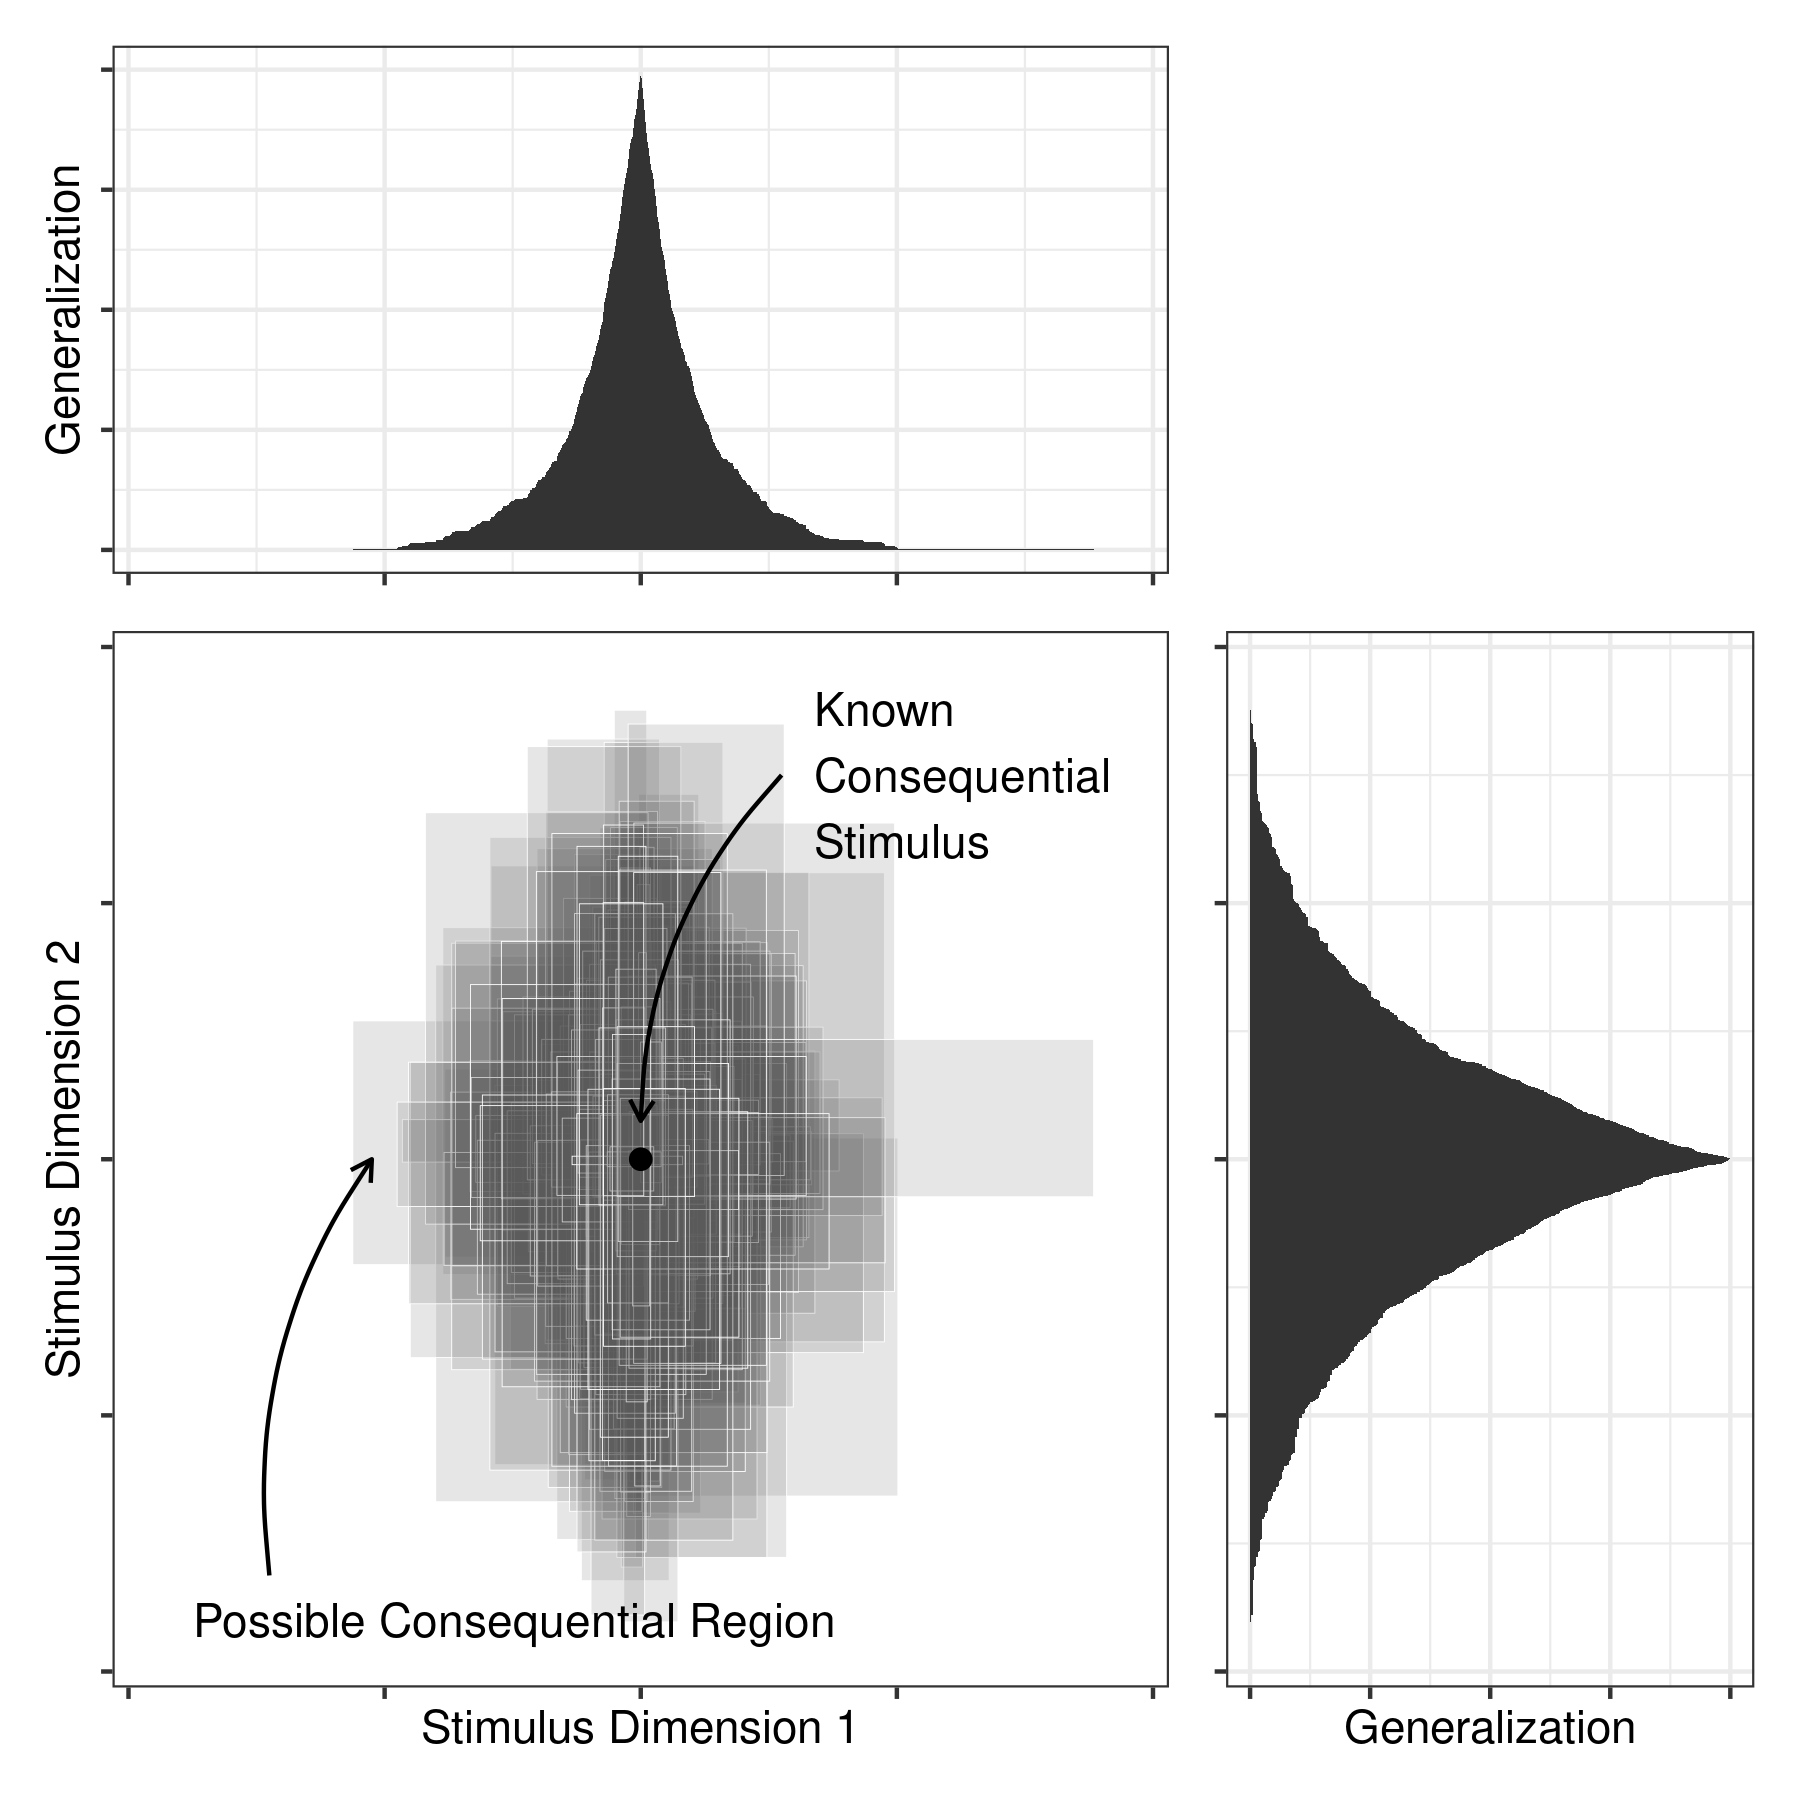
\includegraphics[width=4.5in]{shepardsim} 

}

\caption{A schematic depiction of Shepard's (1987) theory of stimulus generalization. The main panel depicts a two-dimensional psychological space, in which possible stimuli can vary along two stimulus dimensions (e.g., brightness, orientation). The black marker shows the location of a \enquote{consequential stimulus} (e.g., an unpleasant tasting fruit), and each of the grey rectangles represents one possible hypothesis about the range of possible stimuli that might also have this consequence (e.g., taste unpleasant). Not knowing which of these hypotheses represents the true extension of the \enquote{region of unpleasant fruits}, the learner \enquote{averages} across their uncertainty leading to the approximately-exponential generalization gradients plotted above and to the right. Note that the curves shown in this figure are jagged rather than smooth because only a sample of possible regions is depicted, and that for ease of exposition this figure represents a simplified version of Shepard's (1987) theory.}\label{fig:unnamed-chunk-1}
\end{figure}

Although brief, Shepard's paper has been influential in the cognitive science literature. It presented no new empirical data and in substance it is mostly devoted to the derivation of a formal relation between one unobservable quantity (psychological distance) and another (stimulus generalizability). The universal law featured prominently in a special issue of \emph{Brain and Behavior Sciences} in 2001 and a first person retrospective (Shepard, 2004), and for my contribution to this special issue I use it as an example of theory building in psychology.\footnote{It should be noted that I am not going to discuss the empirical evidence for (or against) Shepard's theory. It is not my intent to argue for any specific theory, so much as to describe some of the processes that go into constructing, extending and evaluating one. Most theories are, of course, wrong. I would not be surprised if Shepard's work (or indeed my own) turns out to be misguided. That is not the point of this paper. The point is to present my views on what psychological theories are and how they can be useful.} The decision to focus on a single theoretical contribution is motivated by a desire to look at the particulars rather than speak solely in the abstract; and my decision to ignore disciplines outside of cognitive psychology is motivated by a desire to work toward what Flis (2019) calls \enquote{an indigenous epistemology}. If psychology is to make theoretical progress we must do so on our own terms. There are limits to what we can learn from the physical sciences.

Some desiderata for scientific theories seem easy to list. A scientific theory should be independent of its creator, for instance. It is difficult to make much use of a theory otherwise. In practice this typically means a theory is mathematical or computational in nature. Similarly, psychological theories should of course make some connection with empirical data, giving an account of the generative mechanism that gave rise to those data. Theories should be usable, in the sense of providing other scientists guidance for future research. Other criteria could also be named, including falsifiability, simplicity, compatibility with existing literature, generalizability, predictive ability and so on. However, while it is easy to list desiderata and even easier to argue over which elements to such lists are the most important, such ``discussions in the abstract'' rarely provide much guidance to the would-be theoretician. From the perspective of the working scientist, it is perhaps more useful to give concrete examples, and to that end I return to an examination of Shepard's (1987) paper and the mathematical psychology literature to which it belongs. There are five claims I wish to make: (1) theory building is not a statistical problem; (2) mathematical formalism is theoretically beneficial; (3) measurement and theory have a complex relationship; (4) rewriting old theory can yield new insights; and (5) theoretical growth can drive empirical work that might not otherwise have been considered worthwhile.

\hypertarget{theory-building-is-not-a-statistical-problem}{%
\section{Theory building is not a statistical problem}\label{theory-building-is-not-a-statistical-problem}}

\noindent
Reading Shepard's original 1987 paper and the 2004 retrospective, some surprising characteristics of his theoretical work stand out. First, the theoretical development was largely post hoc. The paper does not collect new data, and indeed the main empirical results reported in the paper were based on a reanalysis of existing data. Second, the paper reports no hypothesis tests. There are no p-values, no Bayes factors, nor any confidence intervals or their Bayesian equivalents. Third, the paper does not outline any specific predictions about future experiments. It makes a strong claim that the exponential law should hold broadly but does not prescribe how tests of this prediction should be constructed.

Viewed through the lens of the methodological reform culture documented by Flis (2019) these properties might seem strange, and might even amount to a form of \enquote{questionable research practice}. For instance, in the current zeitgeist it is sometimes argued with considerable vigor (especially on informal forums such as academic twitter) that strong inferential claims cannot be justified without preregistered confirmatory tests. Shepard's (1987) paper does not present any such tests, but makes sweeping claims nonetheless. Similarly, one might wonder if his post hoc theorizing is a form of hypothesizing after results are known. The unwary reader might conclude that Shepard's work is of questionable value: perhaps cognitive scientists have erred by according this paper such high status?

Something seems awry in this description, and few researchers familiar with Shepard's work would endorse it. The problem, I suggest, arises from a subtle way in which the preceding paragraph misrepresents the inferential problems scientists face. Methodological prescriptions relating to confirmatory tests (e.g.~Wagenmakers, Wetzels, Borsboom, Maas, \& Kievit, 2012) or post hoc hypotheses (e.g.~Kerr, 1998) are narrow in scope: they have been developed to guide \emph{statistical} inferences about empirical data, and as I have argued before (Navarro, 2019) it is an error to presume that the same logic can be applied to the evaluation of \emph{scientific} theories.\footnote{The reader may wonder then if I am constructing a \enquote{strawman} argument by implying that theory building might be dismissed on this basis. All I can say in response is that I have received reviews in recent years (including by open science advocates!) that have accused me of questionable research practice precisely because my \emph{theoretical} work does not meet these statistical criteria. It is easy to claim that no-one would fall prey to the fallacy of conflating statistical with theoretical claims, but it does happen and I believe there is value to pointing out the error in the open literature rather than arguing it invisibly in the review process.} To put it another way, the success of Shepard's (1987) theoretical work in spite of the (apparent) failure to meet these statistical prescriptions tells us something about about what a theory is not. In my view neither empirical data nor statistical tests can be called a theoretical contribution, and prescriptions deemed sensible for empirical research or data analysis should not be considered suitable for the evaluation of psychological theory.

I suggest that the theoretical value in Shepard's paper was not the discovery of an exponential law but rather the \emph{explanation} proposed for it, and theories need to be evaluated (in part) in terms of their explanatory value. For example, Shepard's paper did not merely summarize data, it systematized an existing body of empirical findings. It separated aspects to the data that are invariant across studies from those that are not, sifting the wheat from the chaff so to speak. The sieve that enabled this was a mathematical theory describing regularities in stimulus generalization in terms of simpler primitives. Thus while Shepard's theory asserts that the form of a generalization curve should be exponential, this exponential form is an entailment of his theory and not its substance.

From a theoretical perspective this is important: if an exponential law were observed in a few terrestrial species with no deeper explanation provided, there would be little reason to believe that such a law might hold with any generality. Such inference would be statistically unjustifiable, even as a \enquote{tentative suggestion}. What Shepard does instead is note that an exponential law emerges as an entailment of sufficiently primitive rules that could be reasonably expected to hold in vastly different environments:

\begin{quote}
I tentatively suggest that because these regularites reflect universal principles of natural kinds and of probabilistic geometry, natural selection may favor their increasingly close approximation in sentient organisms wherever they evolve. (Shepard, 1987, p.~1323)
\end{quote}

\noindent
In other words, his claim to generality does not arise from any statistical quantification of the strength of evidence, but from the formal structure of the theory. Statistical evidence and theoretical generality are quite different things. Statistical tools can tell us what we might expect to happen were an experiment to be precisely replicated in precisely the same context; theoretical tools exist to tell us how to generalize from one context to another. Insofar as all meaningful inferences that a practical scientist cares about are to some extent an act of generalization across contexts, statistical inferences are insufficient to guide scientific judgment. Theory-based inferences are a necessity, not a luxury.

\hypertarget{mathematical-formalism-is-theoretically-beneficial}{%
\section{Mathematical formalism is theoretically beneficial}\label{mathematical-formalism-is-theoretically-beneficial}}

\noindent
It is perhaps trite to say so, but the defining property of mathematical psychology is the emphasis on \emph{formal} descriptions of human thought and behavior, either in the form of an abstract mathematical specification or a clearly defined computational model. To many psychologists it might seem strange that such a discipline even exists but as Luce (1995) puts it \enquote{mathematics becomes relevant to science whenever we uncover structure in what we are studying} (p.~2). If we believe that our empirical results have structure we should attempt to articulate what that structure is, as precisely as we are able. It is with this task that mathematical psychology is concerned.

There are a number of reasons why formality is useful to the would-be theoretician, but first among them (in my view) is \emph{precision}. Consider how Shepard's law of generalization might have looked had he not sought the precision that mathematics affords. My attempt to describe the law itself verbally using ordinary English language and not substituting any mathematical words is as follows:

\begin{quote}
If an intelligent agent encounters one thing that has a particular property, and encounters another thing and is uncertain whether it possesses that property, then all else being equal the agent will tend to treat those things similarly in regards to the \emph{unknown} property to the extent that those two things are similar in regards to their \emph{known} properties, and this tendency will fall away very quickly as this similarity decreases
\end{quote}

\noindent
Except for that last part -- which forms the substantive part of the exponential law -- this seems like a commonsense intuition, but in the stated form it also sounds vacuous and perilously close to tautological. What precisely do I mean when I use the word \enquote{similarity}? As philosophers (Goodman, 1972) and psychologists (Medin, Goldstone, \& Gentner, 1993) alike have noted, the term \enquote{similarity} is not well-defined and requires additional constraint to be psychologically meaningful. To make the theory workable, I must elaborate on this verbal definition and try to pin down what I mean by \enquote{similarity}. I will also need to pin down what I mean when I refer to the \enquote{tendency} to act a certain way. Very quickly one finds that it is difficult to work out \emph{what} underlying theoretical claim is being made, if these claims are stated only in everyday language. Even if the theoretical claim is not entirely vacuous -- in this case, if there is some of substance buried within my claim that \enquote{the tendency falls away very quickly} -- I cannot work out what the substance may be when my theory is stated in this fashion. In other words, without precision it is hard to know what tests and what inferences are licensed by the theory.

Escaping this trap of vagueness is hard, and to illustrate how mathematical formalism can help it will be necessary to introduce some.\footnote{It is worth noting that doing so is often viewed as a risky proposition in psychology. In my experience journal editors and reviewers are less likely to accept a paper that contains formal exposition, and will often ask for such things to be removed, relegated to supplementary materials, appendices, or even recommend that papers be \enquote{sent to a more specialist journal}. Though I have been as guilty of this practice as anyone else, I am of the view that the hostility of institutional gatekeepers to mathematical methods in psychology is part of the very problem that needs to be addressed.} In this paper I'll use \(g(x, y)\) to refer to the generalization function: specifically, \(g(x, y)\) is the probability that a newly encountered stimulus \(y\) shares a property that is already known to be possessed by a different stimulus \(x\). Using this notation, Shepard's claim can be written in the following form:

\begin{equation}
g(x, y) = e^{-\lambda \, d(x, y)}
\end{equation}

\noindent
where the constant \(e\) is approximately 2.718 and \(\lambda\) is an unknown parameter of little theoretical interest.\footnote{This is not quite true. The \enquote{specificity} parameter \(\lambda\) describes how quickly the generalization gradient falls away as a function of distance, and there are many situations in which the researcher may care primarily about how \(\lambda\) changes across contexts. However, those situations were not the focus of Shepard's work.} The quantity of interest here is \(d(x, y)\) namely the \enquote{psychological distance} between stimulus \(x\) and stimulus \(y\). Written like this, the theoretical claim starts to become clearer: if it is possible to measure \emph{both} the psychological distance \(d(x, y)\) and the strength of generalization \(g(x, y)\) in a defensible way, then we should expect a very specific non-linear relationship to emerge between the two. Already some of the value of the theory should be clear. It tells us which measurement problems we need to solve.

The value of this should not be understated: knowing what quantities need to be measured is of considerable importance to us as psychologists, and similarly knowing when approximate measurements are \enquote{good enough} is critical. In the generalization context, if the researcher can only obtain ordinal-scale information about psychological distances, then Shepard's law yields \emph{no predictions at all} about the corresponding generalizations. Indeed, to the extent that one goal in methodological reform is to encourage researchers to be more precise in stating the contexts to which we believe our results may generalize (Simons, Shoda, \& Lindsay, 2017), it is to our advantage to have precisely stated theory to guide us. To comment sensibly on how an empirical result might be expected to generalize (or not) beyond the original context, one needs to know something about what properties of the sample or the study are \emph{projectible} in the sense described by Goodman (1955). Formal theory helps by providing the researcher with guidance as to what matters and what does not. Indeed, Shepard's description of the generalization problem facing every learner seems pointedly appropriate to the generality problem facing us as scientists:

\begin{quote}
We generalize from one situation to another not because we cannot tell the difference between the two situations but because we judge that they are likely to belong to a set of situations having the same consequence. Generalization, which stems from uncertainty about the distribution of consequential stimuli in psychological space, is thus to be distinguished from failure of discrimination, which stems from uncertainty about the relative locations of individual stimuli in that space (Shepard 1987, p.~1322)
\end{quote}

\noindent
If we hope to make sound generalizations as scientists, we must know what theoretical space attaches to our empirical work: my modest suggestion is that formal mathematical theories are the method by which we can do so.

\hypertarget{measurement-and-theory-have-a-complicated-relationship}{%
\section{Measurement and theory have a complicated relationship}\label{measurement-and-theory-have-a-complicated-relationship}}

\noindent
Let us turn next to the question of measurement and its relation to theory. If one hopes to obtain empirical support for a theoretical claim, there must be some mechanism by which the theory is tethered in some way to observational or experimental data. To accomplish this, one must have an appropriate measurement tool. For example, one of the key insights in Shepard's (1987) paper is the recognition that stimulus generalization functions are extremely irregular in form when we measure distance in \enquote{objective} terms are often very smooth when measured in more subjective terms: color generalizations are predictable with respect to the appropriate color space (e.g., Ekman, 1954), tones are regular when described in an appropriate perceptual space, etc. In retrospect this seems obvious, but at the time Shepard developed the theory he was faced with a substantive problem of how to extract the \emph{appropriate} stimulus representation to which the theory might be applied. Setting aside the justifications for his choices, nonmetric multidimensional scaling served (MDS; Kruskal, 1964) as a measurement model for Shepard in 1987, and his analyses all use MDS-estimated psychological spaces to supply the relevant measure of distance.

As this discussion illustrates, the measurement instrument and the theoretical development were tightly linked. Without MDS as a measurement tool Shepard would have found it almost impossible to formulate the empirical regularity of interest with any confidence. However, it is equally clear that MDS is merely a tool used to help define the phenomenon to be explained. It can be used to supply an approximate measure of psychological distance \(d(x,y)\) between two stimuli, but it does \emph{not} itself explain why a measure of stimulus generalization \(g(x,y)\) should diminish exponentially as a function of this distance. Though MDS and other latent variable models (e.g., factor analysis) can be useful tools for organizing our measurements in a statistically meaningful way, we ought not mistake them for psychological theory.

To illustrate the latter point, it is notable that in the stimulus generalization literature it quickly became apparent that Shepard's law applies even in situations where MDS does not: shortly after the publication of Shepard's original paper, Russell (1988) demonstrated that the same law holds for stimuli defined in terms of discrete features as well as to the continuous spaces for which Shepard's work was defined, a connection that was later extended by Tenenbaum and Griffiths (2001). While the theoretical framework could not have come into existence without the scaffolding provided by the MDS measurement model, it quickly outgrew any need for this support. Many of the generalization problems discussed by Tenenbaum and Griffiths cannot be described with respect to any metric space extracted by MDS, but are nevertheless consistent with Shepard's theory. In other words, while the measurement model supplied by MDS played a central role in developing theories of generalization, those theories are no longer dependent on MDS in any meaningful sense.

\hypertarget{rewriting-old-theory-can-provide-new-insight}{%
\section{Rewriting old theory can provide new insight}\label{rewriting-old-theory-can-provide-new-insight}}

\noindent
The specific mathematical form that Shepard used to implement his ideas is not unique, and the theory can be rewritten in different notation. Previously, Cooper and Guest (2014) have argued that theoretical work need not be constrained to a particular \enquote{implementation} (or formalism), but is better captured by a more abstract notion of a \enquote{specification}. As a concrete example, it is worth considering the manner in which Shepard's law was later reformulated by Tenenbaum and Griffiths as an (explicitly) Bayesian model, and the effect this rewriting had on how the theory could be applied.

To illustrate what I mean here, it is worth considering how Bayesian cognitive models are typically described in the cognitive science literature. Nowadays it is grossly typical to introduce such a model by first saying \enquote{we propose to treat {[}psychological problem of interest{]} as a Bayesian inference problem}, and then introduce the formula for Bayes' rule:

\begin{equation}
P(h | x) = \frac{P(x | h) P(h)}{P(x)}
\end{equation}

\noindent
It would then be explained that \(P(h)\) defines the learner's \emph{prior} degree of belief in some hypothesis \(h\) about the world, whereas \(P(h|x)\) is the \emph{posterior} belief in that hypothesis after the learner encounters the information embodied by \(x\), whatever \(x\) may happen to be in the specific application at hand. Next it would be noted that the likelihood term \(P(x|h)\) denotes the probability of the learner observing \(x\) if hypothesis \(h\) were true. The normalizing constant \(P(x)\) is also explained, additional context is filled in, and the end result is an abstract specification for a mathematical model.\footnote{A complete discussion of Bayesian cognitive modelling is beyond the scope of this brief paper: see Perfors, Tenenbaum, Griffiths, and Xu (2011) for a tutorial introduction.}

If one reads Shepard's (1987) paper, one finds nothing of the kind. None of the \enquote{standard} notation is used and there is no explicit appeal to Bayes' rule in the text. Instead, all that one one finds is a discussion of \enquote{consequential regions} of unknown size, probability measures that are not entirely easy to understand for the casual reader, and so on. It does not \emph{look} like a Bayesian model in the sense that cognitive modelers would easily recognize 30 years later. I can certainly attest to the fact that I did not perceive the connection to Bayesian learning until Tenenbaum and Griffiths (2001) recast Shepard's formalism using different notation, expressing the same ideas rather differently.

The theoretical contribution of the Tenenbaum and Griffiths (2001) paper is worth expanding on, because I think it was instrumental in allowing Shepard's model to be extended beyond the original stimulus generalization context. Where Shepard referred to the notion of a \enquote{consequential region} located within a psychological space -- with all the geometric connotations that entails -- Tenenbaum and Griffiths took a more general view and framed their analysis in terms of \enquote{consequential sets}. Moreover, any specific candidate for the true consequential set was labeled a \enquote{hypothesis} \(h\) and considered part of a broader \enquote{hypothesis space} \(\mathcal{H}\) and the underlying problem of generalizing from one stimulus to another could be recast as Bayesian reasoning about (collections of) such hypotheses.

The Bayesian reformulation of Shepard's theory presented by Tenenbaum and Griffiths allowed them to generalize Shepard's theory in three distinct ways. First, as mentioned earlier, they showed (much like Russell 1988) that Shepard's theory could encompass stimuli that were not representable as points in a metric space: in their notation, this is as accomplished by substituting a new hypothesis space \(\mathcal{H}\). Second, this formulation allowed the theory to naturally accommodate inductive generalization problems in which the learner has encountered more than one consequential stimulus. Earlier approaches for allowing the model to account for multi-item generalization (e.g., Shepard \& Kannappan, 1991) were not quite so adaptable.

Finally, this formalism called attention to a potentially limiting assumption in Shepard's original paper. Shepard (1987, p.~1321) argued that \enquote{in the absence of any information to the contrary, an individual might best assume that nature selects the consequential region and the first stimulus independently}. This assumption places strong constraints on the inferences that the learner can make, and when formally instantiated within the model it leads to a situation in which the learner necessarily behaves like a naive falsificationist: the only role that observed stimuli \(x\) can play is indicating which hypotheses \(h\) are consistent with the observations and which are not. Nevertheless, this is by no means the only assumption a sensible reasoner might make, and by highlighting Shepard's assumption more clearly, Tenenbaum and Griffiths (2001) allowed later work to explore alternative sampling models that allow the reasoner to use the stimulus information in a more sophisticated manner (e.g.~Shafto, Goodman, \& Griffiths, 2014; Hayes, Banner, Forrester, \& Navarro, 2019). Each of these insights has led to new empirical and theoretical work, point I will expand upon in the next section.

\hypertarget{theoretical-growth-can-drive-experimental-innovation}{%
\section{Theoretical growth can drive experimental innovation}\label{theoretical-growth-can-drive-experimental-innovation}}

\noindent
The final point I want to make pertains to the relationship between theoretical growth and empirical innovation. On occasions, I have heard it suggested that psychology needs to solve our empirical problems first and only then consider how to construct good theory. I am less than convinced by such claims, and hope to illustrate in this section why the two problems go hand in hand, as always using the stimulus generalization theories introduced by Shepard (1987) and Tenenbaum and Griffiths (2001) as my example.

Looking at their paper in retrospect, one of the most important contributions made by the Bayesian formulation adopted by Tenenbaum and Griffiths (2001) is that it allowed the underlying theory to be applied in a much broader range of inductive problems. Shepard's (1987) original construction, though purportedly to be a very general law itself, was formulated with respect to a narrow class of psychological problems: inductive generalization from a single observation. Moreover, because the origins of his work lay in the study of human perception and the animal learning literature, it was not immediately clear --- at least it was not clear to me --- how the theory should be extended to higher order cognition. The reformulation offered by Tenenbaum and Griffiths' paper made it quite apparent that Shepard's original theory is a special case of a broader class of Bayesian generalization models. By abstracting away from the specific problem Shepard's theory sought to explain and casting it in a language (Bayesian inference) that is naturally extensible to new problems, I was able to see how I could extend Shepard's theory on my own.

Perhaps the cleanest example of this interplay in my own research is the work presented by Hayes et al. (2019). That paper was motivated by a puzzling finding presented by Lawson and Kalish (2009) in which people appeared to solve inductive reasoning problems differently depending on how the information in the reasoning problem was selected. At the time the original work was presented, no clear explanation for why people would do this was available, so we considered the possibility that --- following Tenenbaum and Griffiths' (2001) observation that from a statistical learning perspective inductive generalization ought to depend on the learner's beliefs about how information is selected --- the earlier results by Lawson and Kalish (2009) were the same kind of effect that their theory predicted.

The process I followed when adapting the theory to a new context may be informative. In my first pass at adapting the theory (Hayes, Banner, \& Navarro, 2017), I constructed a model that was only very slightly different from the Tenenbaum and Griffiths version, and used it to derive qualitative predictions regarding what kind of empirical manipulations should be expected to modulate the effect reported by Lawson and Kalish (2009). We then undertook a series of experimental tests, reported by Hayes et al. (2019) showing that under some circumstances (not all) the effects predicted by (my trivial adaptation of) the Tenenbaum and Griffiths model occur almost exactly as expected. However, from my perspective this initial work was unsatisfying: because our new experimental results involved a very different design to the kind of \enquote{stimulus generalization} tasks with which Shepard was originally concerned, it was difficult to be certain \emph{which} aspects of our data could be explained as a \enquote{sampling effect} and which could not. This led me to a develop a more substantive modification of Tenenbaum and Griffiths' model,\footnote{Crudely put, I modified the hypothesis space \(\mathcal{H}\): instead of each \(h\) corresponding to a single \enquote{consequential set} indicating which stimuli possess an unknown property, the Hayes et al. (2019) model is probabilistic, and a hypothesis \(h\) is a function defined over the stimulus space that describes the \emph{probability} with which stimuli possess an unknown property.} and following the model evaluation procedure outlined in Navarro (2019) I was able to resolve much of this uncertainty: most of our experimental findings were indeed consistent with the theory, but some were emphatically not. By adopting a mathematically precise, theoretically motivated approach to exploring this phenomenon, we were able to obtain clarity about what we were seeing in our empirical data. I know of no other process that would have allowed me to do so.

\hypertarget{a-word-of-warning}{%
\section{A word of warning}\label{a-word-of-warning}}

\noindent
In this paper I have argued that the toolkit provided by mathematical psychology can be a powerful aid to those seeking to build psychological theories. I would be remiss, however, if I did not comment on the limitations to this approach. As a mathematical psychologist studying human inductive reasoning what I \emph{want} is a \enquote{mathematical theory of human reason} that explains the entire psychological process of human reasoning about underconstrained problems. However, my skill and knowledge are both limited and I cannot fathom what class of theoretical models might be applicable to the entire psychological process at hand. Nor can I think of a way to circumscribe the scientific problem in a fashion that allows me render the entire domain of human reason subject to any kind of direct measurement. This limitation has consequences. My experiment is a measurement tool that captures some aspects to human reasoning, but inevitably confounds it with the measurement of some other phenomena. If I try to theoretically account for all things in my data I must provide an account of these unknown things as well as the thing I am trying to study. But if my experiment is too complex then these unknown things will themselves become quite complex, leading to the risk that any theoretical explanation I construct is little more than wild speculation.

One answer to the problem is to make the task simpler. Make the task so small and so simple that we actually can write down models that specify precise assumptions about every aspect to the task. This may lead to better models, but at the price of limiting their theoretical scope to an unreasonable extent. It is inconvenient, perhaps, but it remains true that our models are defined with respect to simplified \enquote{toy worlds}; humans, however, must occupy the real one. If we emphasize formal rigor \emph{too} much, the experimental paradigms may become ossified and highly restricted, adapted to suit only those phenomena that we know how to model in full. This can be dangerous, insofar as it provides an illusion of explanatory power, one that falls apart once we step outside the narrow confines of our paradigm. Hacking (1992) argues that over time laboratory sciences can create a self-vindicating system by building theories and methods that are \enquote{mutually adjusted to each other} and cannot be falsified, quite irrespective of their real world utility:

\begin{quote}
The theories of the laboratory sciences are not directly compared to \enquote{the world}; they persist because they are true to phenomena produced or even created by apparatus in the laboratory and are measured by instruments we have engineered.
\end{quote}

\noindent
Psychologists should not shy away from the theoretical concerns this raises. When seeking to develop theories one should take some care to reflect on how the theoretical perspective may serve to circumscribe the problem at hand in too narrow a way. Precisely because of the fact that mathematical models are hard to build, those of us who advocate formally modelling human thought and behaviour must, I suggest, be especially wary of this trap.

\hypertarget{conclusion}{%
\section{Conclusion}\label{conclusion}}

\noindent
Mathematical psychology is something of an oddity in the discipline. It does not eschew empirical research, but neither does it view the goal of psychological science to be the accrual of empirical effects. Quite unlike most areas of psychology with which I am familiar, mathematical psychologists place a high value on theoretical development, particularly when such theories can be stated in a formal manner. My goal in this paper was to highlight the manner in which cumulative theoretical work has developed in this discipline, using Shepard's law as an example. From its origins in associative learning and stimulus generalization, to its reformulation as a Bayesian model and its extension to a variety of novel contexts, a single theoretical claim can be shown to connect to a variety of empirical findings in superficially distinct domains.

Although I have focused on Shepard's law and its extensions in this paper, I suspect that the underlying pattern is quite general. I could have chosen the Rescorla-Wagner model of associative learning as the basis for this discussion (Rescorla \& Wagner, 1972), or the Generalized Context Model of human categorization (Nosofsky, 1986). I could have chosen to focus on models such as ALCOVE that sought to unify associative learning and categorization (Kruschke, 1992), or models such as the hierarchical Dirichlet process that sought to unify various category learning models within a common theoretical language (Griffiths, Canini, Sanborn, \& Navarro, 2007). I could have revisited Ebbinghaus' 1885 work on memory (reprinted as Ebbinghaus, 2013). I could have examined sequential sampling models of choice reaction time (Luce, 1986) and the rich theoretical tradition that mathematical psychologists have developed in that domain also. In each of these areas psychologists have been slowly and carefully building psychological theories. The work is painstaking and slow, and the papers often difficult to read, but I would argue that the theoretical development in this domain has been genuinely cumulative.

These theoretical advances have something in common. In each of these areas psychological researchers have built up a considerable body of theoretical knowledge that is instantiated in formal models of psychological processes. In every case the underlying theoretical models are more than mere summaries of empirical results, and more substantive than a mere statistical model. In all cases the formalism can be used to generate novel predictions in experimental paradigms that differ markedly from the experimental contexts used to develop the model (and, remarkably, some of those predictions have even turned out to be correct). By a judicious combination of abstraction and formalism, mathematical psychologists have been able to develop a toolkit that allows anyone to derive theoretical predictions in completely novel paradigms. If it is indeed the case that psychology suffers from a kind of ``theoretical amnesia'' (Borsboom, 2013), perhaps the machinery of mathematical psychology can aid its memory. Perhaps fittingly, the words of Shepard (1987, p.~1323) seem an appropriate way to conclude

\begin{quote}
\emph{Undoubtedly, psychological science has lagged by behind physical science by at least 300 years. Undoubtedly, too, prediction of behavior can never attain the precision for animate that it has for celestial bodies. Yet, psychology may not be inherently limited merely to the descriptive characterization of the behaviors of particular terrestrial species. Possibly, behind the diverse behaviors of humans and animals, as behind the various motions of planets and stars, we may discern the operation of universal laws}
\end{quote}

\hypertarget{references}{%
\section{References}\label{references}}

\hypertarget{refs}{}
\leavevmode\hypertarget{ref-boorsbaum2013theoretical}{}%
Borsboom, D. (2013). Theoretical amnesia. \emph{Center for Open Science}. Retrieved from \url{http://osc.centerforopenscience.org/2013/11/20/theoretical-amnesia/}

\leavevmode\hypertarget{ref-cooper2014implementations}{}%
Cooper, R. P., \& Guest, O. (2014). Implementations are not specifications: Specification, replication and experimentation in computational cognitive modeling. \emph{Cognitive Systems Research}, \emph{27}, 42--49.

\leavevmode\hypertarget{ref-ebbinghaus2013memory}{}%
Ebbinghaus, H. (2013). Memory: A contribution to experimental psychology. \emph{Annals of Neurosciences}, \emph{20}(4), 155.

\leavevmode\hypertarget{ref-ekman1954dimensions}{}%
Ekman, G. (1954). Dimensions of color vision. \emph{The Journal of Psychology}, \emph{38}(2), 467--474.

\leavevmode\hypertarget{ref-Flis2019}{}%
Flis, I. (2019). Psychologists psychologizing scientific psychology: An epistemological reading of the replication crisis. \emph{Theory \& Psychology}, \emph{29}(2), 158--181.

\leavevmode\hypertarget{ref-goodman1955new}{}%
Goodman, N. (1955). The new riddle of induction. In \emph{Fact, fiction and forecast}. Harvard University Press.

\leavevmode\hypertarget{ref-goodman1972seven}{}%
Goodman, N. (1972). Seven strictures on similarity. In \emph{Problems and projects}. Bobbs-Merrill.

\leavevmode\hypertarget{ref-griffiths2007unifying}{}%
Griffiths, T., Canini, K., Sanborn, A., \& Navarro, D. (2007). Unifying rational models of categorization via the hierarchical Dirichlet process. In D. S. McNamara \& J. G. Trafton (Eds.), \emph{Proceedings of the 29th annual conference of the cognitive science society} (pp. 323--328). Psychology Press.

\leavevmode\hypertarget{ref-hacking1992self}{}%
Hacking, I. (1992). The self-vindication of the laboratory sciences. In A. Pickering (Ed.), \emph{Science as practice and culture}. University of Chicago Press.

\leavevmode\hypertarget{ref-hayes2019selective}{}%
Hayes, B. K., Banner, S., Forrester, S., \& Navarro, D. J. (2019). Selective sampling and inductive inference: Drawing inferences based on observed and missing evidence. \emph{Cognitive Psychology}, \emph{113}, 101221.

\leavevmode\hypertarget{ref-hayes2017sampling}{}%
Hayes, B. K., Banner, S., \& Navarro, D. J. (2017). Sampling frames, Bayesian inference and inductive reasoning. In G. Gunzelmann, A. Howes, T. Tenbrink, \& E. J. Davelaar (Eds.), \emph{Proceedings of the 39th annual conference of the cognitive science society} (pp. 488--493). Austin, TX: Cognitive Science Society.

\leavevmode\hypertarget{ref-kerr1998harking}{}%
Kerr, N. L. (1998). HARKing: Hypothesizing after the results are known. \emph{Personality and Social Psychology Review}, \emph{2}(3), 196--217.

\leavevmode\hypertarget{ref-kruschke1992alcove}{}%
Kruschke, J. K. (1992). ALCOVE: An exemplar-based connectionist model of category learning. \emph{Psychological Review}, \emph{99}(1), 22--44.

\leavevmode\hypertarget{ref-kruskal1964nonmetric}{}%
Kruskal, J. B. (1964). Nonmetric multidimensional scaling: A numerical method. \emph{Psychometrika}, \emph{29}(2), 115--129.

\leavevmode\hypertarget{ref-lawson2009sample}{}%
Lawson, C. A., \& Kalish, C. W. (2009). Sample selection and inductive generalization. \emph{Memory \& Cognition}, \emph{37}(5), 596--607.

\leavevmode\hypertarget{ref-luce1986response}{}%
Luce, R. D. (1986). \emph{Response times: Their role in inferring elementary mental organization}. Oxford University Press.

\leavevmode\hypertarget{ref-luce1995four}{}%
Luce, R. D. (1995). Four tensions concerning mathematical modeling in psychology. \emph{Annual Review of Psychology}, \emph{46}(1), 1--27.

\leavevmode\hypertarget{ref-medin1993respects}{}%
Medin, D. L., Goldstone, R. L., \& Gentner, D. (1993). Respects for similarity. \emph{Psychological Review}, \emph{100}(2), 254--278.

\leavevmode\hypertarget{ref-navarro2019between}{}%
Navarro, D. J. (2019). Between the devil and the deep blue sea: Tensions between scientific judgement and statistical model selection. \emph{Computational Brain \& Behavior}, \emph{2}(1), 28--34.

\leavevmode\hypertarget{ref-nosofsky1986attention}{}%
Nosofsky, R. M. (1986). Attention, similarity, and the identification--categorization relationship. \emph{Journal of Experimental Psychology: General}, \emph{115}(1), 39--57.

\leavevmode\hypertarget{ref-perfors2011tutorial}{}%
Perfors, A., Tenenbaum, J. B., Griffiths, T. L., \& Xu, F. (2011). A tutorial introduction to Bayesian models of cognitive development. \emph{Cognition}, \emph{120}(3), 302--321.

\leavevmode\hypertarget{ref-rescorla1972theory}{}%
Rescorla, R. A., \& Wagner, A. R. (1972). A theory of pavlovian conditioning: Variations in the effectiveness of reinforcement and nonreinforcement. \emph{Classical Conditioning II: Current Research and Theory}, \emph{2}, 64--99.

\leavevmode\hypertarget{ref-russell1988analogy}{}%
Russell, S. (1988). Analogy by similarity. In D. H. Helman (Ed.), \emph{Analogical reasoning} (pp. 251--269). Springer.

\leavevmode\hypertarget{ref-shafto2014rational}{}%
Shafto, P., Goodman, N. D., \& Griffiths, T. L. (2014). A rational account of pedagogical reasoning: Teaching by, and learning from, examples. \emph{Cognitive Psychology}, \emph{71}, 55--89.

\leavevmode\hypertarget{ref-shepard1987toward}{}%
Shepard, R. N. (1987). Toward a universal law of generalization for psychological science. \emph{Science}, \emph{237}(4820), 1317--1323.

\leavevmode\hypertarget{ref-shepard2004cognitive}{}%
Shepard, R. N. (2004). How a cognitive psychologist came to seek universal laws. \emph{Psychonomic Bulletin \& Review}, \emph{11}(1), 1--23.

\leavevmode\hypertarget{ref-shepard1991toward}{}%
Shepard, R. N., \& Kannappan, S. (1991). Toward a connectionist implementation of a theory of generalization. \emph{Advances in Neural Information Processing Systems}, \emph{3}, 665--671.

\leavevmode\hypertarget{ref-simons2017constraints}{}%
Simons, D. J., Shoda, Y., \& Lindsay, D. S. (2017). Constraints on generality (cog): A proposed addition to all empirical papers. \emph{Perspectives on Psychological Science}, \emph{12}(6), 1123--1128.

\leavevmode\hypertarget{ref-tenenbaum2001generalization}{}%
Tenenbaum, J. B., \& Griffiths, T. L. (2001). Generalization, similarity, and bayesian inference. \emph{Behavioral and Brain Sciences}, \emph{24}(4), 629--640.

\leavevmode\hypertarget{ref-Wagenmakers2012}{}%
Wagenmakers, E.-J., Wetzels, R., Borsboom, D., Maas, H. L. van der, \& Kievit, R. A. (2012). An agenda for purely confirmatory research. \emph{Perspectives on Psychological Science}, \emph{7}, 632--638.

\end{document}
